% Options for packages loaded elsewhere
\PassOptionsToPackage{unicode}{hyperref}
\PassOptionsToPackage{hyphens}{url}
\PassOptionsToPackage{dvipsnames,svgnames,x11names}{xcolor}
%
\documentclass[
]{article}
\usepackage{amsmath,amssymb}
\usepackage{iftex}
\ifPDFTeX
  \usepackage[T1]{fontenc}
  \usepackage[utf8]{inputenc}
  \usepackage{textcomp} % provide euro and other symbols
\else % if luatex or xetex
  \usepackage{unicode-math} % this also loads fontspec
  \defaultfontfeatures{Scale=MatchLowercase}
  \defaultfontfeatures[\rmfamily]{Ligatures=TeX,Scale=1}
\fi
\usepackage{lmodern}
\ifPDFTeX\else
  % xetex/luatex font selection
\fi
% Use upquote if available, for straight quotes in verbatim environments
\IfFileExists{upquote.sty}{\usepackage{upquote}}{}
\IfFileExists{microtype.sty}{% use microtype if available
  \usepackage[]{microtype}
  \UseMicrotypeSet[protrusion]{basicmath} % disable protrusion for tt fonts
}{}
\makeatletter
\@ifundefined{KOMAClassName}{% if non-KOMA class
  \IfFileExists{parskip.sty}{%
    \usepackage{parskip}
  }{% else
    \setlength{\parindent}{0pt}
    \setlength{\parskip}{6pt plus 2pt minus 1pt}}
}{% if KOMA class
  \KOMAoptions{parskip=half}}
\makeatother
\usepackage{xcolor}
\usepackage[margin=1in]{geometry}
\usepackage{color}
\usepackage{fancyvrb}
\newcommand{\VerbBar}{|}
\newcommand{\VERB}{\Verb[commandchars=\\\{\}]}
\DefineVerbatimEnvironment{Highlighting}{Verbatim}{commandchars=\\\{\}}
% Add ',fontsize=\small' for more characters per line
\usepackage{framed}
\definecolor{shadecolor}{RGB}{248,248,248}
\newenvironment{Shaded}{\begin{snugshade}}{\end{snugshade}}
\newcommand{\AlertTok}[1]{\textcolor[rgb]{0.94,0.16,0.16}{#1}}
\newcommand{\AnnotationTok}[1]{\textcolor[rgb]{0.56,0.35,0.01}{\textbf{\textit{#1}}}}
\newcommand{\AttributeTok}[1]{\textcolor[rgb]{0.13,0.29,0.53}{#1}}
\newcommand{\BaseNTok}[1]{\textcolor[rgb]{0.00,0.00,0.81}{#1}}
\newcommand{\BuiltInTok}[1]{#1}
\newcommand{\CharTok}[1]{\textcolor[rgb]{0.31,0.60,0.02}{#1}}
\newcommand{\CommentTok}[1]{\textcolor[rgb]{0.56,0.35,0.01}{\textit{#1}}}
\newcommand{\CommentVarTok}[1]{\textcolor[rgb]{0.56,0.35,0.01}{\textbf{\textit{#1}}}}
\newcommand{\ConstantTok}[1]{\textcolor[rgb]{0.56,0.35,0.01}{#1}}
\newcommand{\ControlFlowTok}[1]{\textcolor[rgb]{0.13,0.29,0.53}{\textbf{#1}}}
\newcommand{\DataTypeTok}[1]{\textcolor[rgb]{0.13,0.29,0.53}{#1}}
\newcommand{\DecValTok}[1]{\textcolor[rgb]{0.00,0.00,0.81}{#1}}
\newcommand{\DocumentationTok}[1]{\textcolor[rgb]{0.56,0.35,0.01}{\textbf{\textit{#1}}}}
\newcommand{\ErrorTok}[1]{\textcolor[rgb]{0.64,0.00,0.00}{\textbf{#1}}}
\newcommand{\ExtensionTok}[1]{#1}
\newcommand{\FloatTok}[1]{\textcolor[rgb]{0.00,0.00,0.81}{#1}}
\newcommand{\FunctionTok}[1]{\textcolor[rgb]{0.13,0.29,0.53}{\textbf{#1}}}
\newcommand{\ImportTok}[1]{#1}
\newcommand{\InformationTok}[1]{\textcolor[rgb]{0.56,0.35,0.01}{\textbf{\textit{#1}}}}
\newcommand{\KeywordTok}[1]{\textcolor[rgb]{0.13,0.29,0.53}{\textbf{#1}}}
\newcommand{\NormalTok}[1]{#1}
\newcommand{\OperatorTok}[1]{\textcolor[rgb]{0.81,0.36,0.00}{\textbf{#1}}}
\newcommand{\OtherTok}[1]{\textcolor[rgb]{0.56,0.35,0.01}{#1}}
\newcommand{\PreprocessorTok}[1]{\textcolor[rgb]{0.56,0.35,0.01}{\textit{#1}}}
\newcommand{\RegionMarkerTok}[1]{#1}
\newcommand{\SpecialCharTok}[1]{\textcolor[rgb]{0.81,0.36,0.00}{\textbf{#1}}}
\newcommand{\SpecialStringTok}[1]{\textcolor[rgb]{0.31,0.60,0.02}{#1}}
\newcommand{\StringTok}[1]{\textcolor[rgb]{0.31,0.60,0.02}{#1}}
\newcommand{\VariableTok}[1]{\textcolor[rgb]{0.00,0.00,0.00}{#1}}
\newcommand{\VerbatimStringTok}[1]{\textcolor[rgb]{0.31,0.60,0.02}{#1}}
\newcommand{\WarningTok}[1]{\textcolor[rgb]{0.56,0.35,0.01}{\textbf{\textit{#1}}}}
\usepackage{graphicx}
\makeatletter
\def\maxwidth{\ifdim\Gin@nat@width>\linewidth\linewidth\else\Gin@nat@width\fi}
\def\maxheight{\ifdim\Gin@nat@height>\textheight\textheight\else\Gin@nat@height\fi}
\makeatother
% Scale images if necessary, so that they will not overflow the page
% margins by default, and it is still possible to overwrite the defaults
% using explicit options in \includegraphics[width, height, ...]{}
\setkeys{Gin}{width=\maxwidth,height=\maxheight,keepaspectratio}
% Set default figure placement to htbp
\makeatletter
\def\fps@figure{htbp}
\makeatother
\usepackage{soul}
\setlength{\emergencystretch}{3em} % prevent overfull lines
\providecommand{\tightlist}{%
  \setlength{\itemsep}{0pt}\setlength{\parskip}{0pt}}
\setcounter{secnumdepth}{-\maxdimen} % remove section numbering
\ifLuaTeX
  \usepackage{selnolig}  % disable illegal ligatures
\fi
\IfFileExists{bookmark.sty}{\usepackage{bookmark}}{\usepackage{hyperref}}
\IfFileExists{xurl.sty}{\usepackage{xurl}}{} % add URL line breaks if available
\urlstyle{same}
\hypersetup{
  pdftitle={Lab 2},
  colorlinks=true,
  linkcolor={Maroon},
  filecolor={Maroon},
  citecolor={Blue},
  urlcolor={blue},
  pdfcreator={LaTeX via pandoc}}

\title{Lab 2}
\author{}
\date{\vspace{-2.5em}Math 241, Week 2}

\begin{document}
\maketitle

\begin{Shaded}
\begin{Highlighting}[]
\CommentTok{\# Put all necessary libraries here}
\CommentTok{\# I got you started!}
\CommentTok{\# The first time you want to install the dsbox package; then you can comment it out.}
\CommentTok{\# If you have not installed the devtools package, you will need to do so first}
\CommentTok{\# install.packages("devtools")}
\CommentTok{\# library(devtools)}

\NormalTok{devtools}\SpecialCharTok{::}\FunctionTok{install\_github}\NormalTok{(}\StringTok{"tidyverse/dsbox"}\NormalTok{)}
\FunctionTok{library}\NormalTok{(dsbox)}
\FunctionTok{library}\NormalTok{(tidyverse)}
\FunctionTok{library}\NormalTok{(viridis)}
\end{Highlighting}
\end{Shaded}

\hypertarget{due-thursday-february-8th-at-830am}{%
\subsection{Due: Thursday, February 8th at
8:30am}\label{due-thursday-february-8th-at-830am}}

\hypertarget{goals-of-this-lab}{%
\subsection{Goals of this lab}\label{goals-of-this-lab}}

\begin{enumerate}
\def\labelenumi{\arabic{enumi}.}
\tightlist
\item
  Practice coding to adhere to the Tidyverse Style Guide.
\item
  Practice creating and refining graphs with \texttt{ggplot2}.
\item
  Consider the strengths and weaknesses of various \texttt{geom}s and
  \texttt{aes}thetics for telling a data story.
\end{enumerate}

\hypertarget{notes}{%
\subsection{Notes:}\label{notes}}

\begin{itemize}
\tightlist
\item
  When creating your graphs, consider context (i.e.~axis labels, title,
  \ldots)!
\item
  If I provide partially completed code, I will put
  \texttt{eval\ =\ FALSE} in the chunk. Make sure to change that to
  \texttt{eval\ =\ TRUE} once you have completed the code in the chunk.
\item
  Be prepared to ask for help from me, Simon, and your classmates! We
  scratched the surface of \texttt{ggplot2} in class. But I encourage
  you to really dig in and make your graphs your own (i.e.~don't rely on
  defaults).
\end{itemize}

\hypertarget{problems}{%
\subsection{Problems}\label{problems}}

\hypertarget{probem-1-road-traffic-injuries-in-edinburgh-scotland}{%
\subsubsection{Probem 1: Road traffic injuries in Edinburgh,
Scotland}\label{probem-1-road-traffic-injuries-in-edinburgh-scotland}}

The dataset can be found in the \texttt{dsbox} package, and is called
\texttt{accidents}. It covers all recorded accidents in Edinburgh in
2018; compared to the dataset made available by the UK government, some
of the variables were modified for the purposes of the package. You can
find out more about the dataset by inspecting its documentation with
\texttt{?accidents}. Recreate the following plot, and interpret the
results.

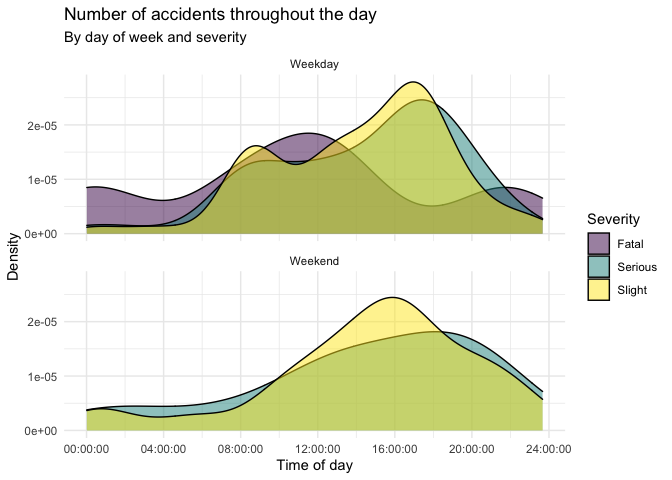
\includegraphics[width=1\linewidth]{../img/edi-accidents-1}

\hypertarget{problem-2-one-dataset-visualized-25-5-ways}{%
\subsubsection{\texorpdfstring{Problem 2: One Dataset, Visualized
\st{25} 5
Ways}{Problem 2: One Dataset, Visualized 25 5 Ways}}\label{problem-2-one-dataset-visualized-25-5-ways}}

Inspired by Nathan Yau's
\href{https://flowingdata.com/2017/01/24/one-dataset-visualized-25-ways/}{One
Dataset, Visualized 25 Ways}, I want you to create 5 visualizations of
the same data. You can use the \texttt{mpg} dataset or another dataset
of your choosing, including the \texttt{accidents} dataset above. Make
sure you have the data manual open for this problem!

\begin{enumerate}
\def\labelenumi{\alph{enumi}.}
\item
  Pick 3 - 4 variables you want to explore. Provide their code names
  here.
\item
  Create 5 graphs. A few things to consider:

  \begin{itemize}
  \tightlist
  \item
    Like Nathan's graphs, they don't all have to contain every one of
    your selected variables.
  \item
    You can't use the same \texttt{geom} for all four graphs but you can
    use the same \texttt{geom} more than once.
  \item
    Think carefully about color, the coordinate system, and scales.
  \item
    Feel free to subset or wrangling the dataset if you want to but it
    isn't required.
  \end{itemize}
\item
  Discuss the pros/cons of your graphs. What useful information can be
  gleaned? How do the different geoms and aesthetics impact the story?
\end{enumerate}

\hypertarget{problem-3-style-this-code}{%
\subsubsection{Problem 3: Style This
Code!}\label{problem-3-style-this-code}}

Take the following code and don't change its functionality but DO change
its style. Use the \href{https://style.tidyverse.org/}{Tidyverse Style
Guide}!

\begin{Shaded}
\begin{Highlighting}[]
\NormalTok{thing}\FloatTok{.132232}\OtherTok{=}\FunctionTok{data.frame}\NormalTok{(}\AttributeTok{theanimalsweightisthisnumber=}\FunctionTok{c}\NormalTok{(}\FunctionTok{runif}\NormalTok{(}\DecValTok{3}\NormalTok{),}\ConstantTok{NA}\NormalTok{),}\AttributeTok{y=}\FunctionTok{c}\NormalTok{(}\StringTok{"cat"}\NormalTok{,}\StringTok{"mouse"}\NormalTok{,}\StringTok{"dog"}\NormalTok{,}\StringTok{"rat"}\NormalTok{))}
\FunctionTok{median}\NormalTok{(thing}\FloatTok{.132232}\SpecialCharTok{$}\NormalTok{theanimalsweightisthisnumber, }\ConstantTok{TRUE}\NormalTok{);}\FunctionTok{mean}\NormalTok{(thing}\FloatTok{.132232}\SpecialCharTok{$}\NormalTok{theanimalsweightisthisnumber, }\DecValTok{0}\NormalTok{ , }\ConstantTok{TRUE}\NormalTok{); }\FunctionTok{var}\NormalTok{(thing}\FloatTok{.132232}\SpecialCharTok{$}\NormalTok{theanimalsweightisthisnumber, }\ConstantTok{NULL}\NormalTok{, }\ConstantTok{TRUE}\NormalTok{)}
\end{Highlighting}
\end{Shaded}

\begin{verbatim}
## [1] 0.8804867
\end{verbatim}

\begin{verbatim}
## [1] 0.8229783
\end{verbatim}

\begin{verbatim}
## [1] 0.02363037
\end{verbatim}

\begin{Shaded}
\begin{Highlighting}[]
\FunctionTok{ggplot}\NormalTok{(thing}\FloatTok{.132232}\NormalTok{, }\FunctionTok{aes}\NormalTok{(}\AttributeTok{y=}\NormalTok{theanimalsweightisthisnumber,}\AttributeTok{x=}\NormalTok{y))}\SpecialCharTok{+}\FunctionTok{geom\_col}\NormalTok{()}\SpecialCharTok{+}\FunctionTok{scale\_y\_continuous}\NormalTok{()}
\end{Highlighting}
\end{Shaded}

\includegraphics{lab02_files/figure-latex/unnamed-chunk-3-1.pdf}

\hypertarget{problem-4-imitation-is-the-sincerest-form-of-flattery}{%
\subsubsection{Problem 4: Imitation is the Sincerest Form of
Flattery}\label{problem-4-imitation-is-the-sincerest-form-of-flattery}}

For this problem, I want you to try to recreate a FiveThirtyEight.com
graphic. Awesomely, they share their data with the world
\href{https://data.fivethirtyeight.com/}{here}. (Note: You don't need to
recreate all their branding/background color scheme.)

\begin{enumerate}
\def\labelenumi{\alph{enumi}.}
\item
  Take a screenshot of the graph, upload it to the same folder on the
  server where you have saved your lab, and insert the file name below.
  Then change the \texttt{eval\ =\ FALSE} to \texttt{eval\ =\ TRUE}.
\item
  Load the data and recreate the graph as best as you can.
\item
  Now make the graph better somehow.
\item
  Justify why your rendition of this \texttt{FiveThirtyEight.com} graph
  is more effective at telling the data story than the original.
\end{enumerate}

\hypertarget{problem-5-rental-apartments-in-sf}{%
\subsubsection{Problem 5: Rental apartments in
SF}\label{problem-5-rental-apartments-in-sf}}

The data for this exercise comes from \texttt{TidyTuesday}, and is on
rental prices in San Francisco. You can find out more about the dataset
by inspecting its documentation
\href{https://github.com/rfordatascience/tidytuesday/tree/master/data/2022/2022-07-05}{here}.
The dataset you'll be using is called \texttt{rent}. Create a
visualization that will help you compare the distribution of rental
prices (\texttt{price}) per bedroom (\texttt{beds}) across neighborhoods
(\texttt{nhood}) in the city of San Francisco
\texttt{(city\ ==\ "san\ francisco")}, over time.

Limit your analysis to rentals where the full unit is available,
i.e.~(\texttt{room\_in\_apt\ ==\ 0}). You have the flexibility to choose
which years and which neighborhoods. Note that you should have a maximum
of 8 neighborhoods on your visualization, but one or more of them can be
a combination of many (e.g., an ``other'' category). Your visualization
should also display some measure of the variability in your data. You
get to decide what type of visualization to create and there is more
than one correct answer! In your answer, include a brief description of
why you made the choices you made as well as an interpretation of the
findings of how rental prices vary over time and neighborhoods in San
Francisco.

\begin{Shaded}
\begin{Highlighting}[]
\CommentTok{\# Get the Data}

\CommentTok{\# Read in with tidytuesdayR package }
\CommentTok{\# Install from CRAN via: install.packages("tidytuesdayR")}
\CommentTok{\# This loads the readme and all the datasets for the week of interest}

\FunctionTok{library}\NormalTok{(tidytuesdayR)}
\NormalTok{tuesdata }\OtherTok{\textless{}{-}}\NormalTok{ tidytuesdayR}\SpecialCharTok{::}\FunctionTok{tt\_load}\NormalTok{(}\StringTok{\textquotesingle{}2022{-}07{-}05\textquotesingle{}}\NormalTok{) }\CommentTok{\# this could take a minute}

\NormalTok{rent }\OtherTok{\textless{}{-}}\NormalTok{ tuesdata}\SpecialCharTok{$}\NormalTok{rent}
\end{Highlighting}
\end{Shaded}


\end{document}
